\subsection{Initial conditions}
In the solution of the KS-equation periodic boundary conditions were implemented, i.e. $u(0,t) = u(L,t)$, as well as $L$-periodic initial conditions. A common initial condition used in several other reports is

\begin{equation}
\label{initialCondition}
u(x,0) = \cos(\frac{x}{16})(1 + \sin(\frac{x}{16})),
\end{equation}

where $x = [0, 32\pi]$ is the space-interval. Another initial condition is

\begin{equation}
\label{initialCondition2}
u(x,0) = \frac{1}{\sqrt{2}} \sin(x) - \frac{1}{8}\sin(2x),
\end{equation}

on the space-interval $x = [0, 2\pi]$, which worked well. The L-periodic initial conditions are customarily taken \cite{periodicInitial} to satisfy

\begin{equation}
\int_0^L\! f(x)\,\textrm{d}x = 0,
\end{equation} 
which both \eqref{initialCondition} and \eqref{initialCondition2} satisfy. The same article also states that for L-periodic initial data, a unique solution for \eqref{KSeq} exits, and is bounded as $t\rightarrow\infty$. The bound has been proven to be smaller than $O(L^{8/5})$. In the numerical tests, with $t=5000$, the initial condition \eqref{initialCondition} did indeed not exceed the bound, nor did \eqref{initialCondition2}.

\subsection{Reference solution}
As the Kuramoto-Sivashinsky equation does not have an analytical solution, a reference solution was implemented using the ode15s-solver in MATLAB. This solver is especially good for solving stiff differential equations, and it uses an implicit method. Ode15s uses a semi-discretized version of the scheme, where it is discretized in space, but not in time. Hence the length of the time steps varies. The time steps are small when the solution changes rapidly, and larger when the changes in the solution are small. Because the solution is needed at given times to be able to compare it with our numerical solution, we specify the time vector. That does not mean that the solver takes a step length $k$, but rather that it returns a solution with step length $k$, with the same accuracy as the computed time points. \cite{ode15s}


\subsection{Results from the IMEX-scheme}
The IMEX method produced figure \ref{fig:surface}. It is easy to see that the solution is chaotic, and the figure shows in a good way that small variations in space leads to large variations in the solution $u(x,t)$.

\begin{figure}[H]
\centering
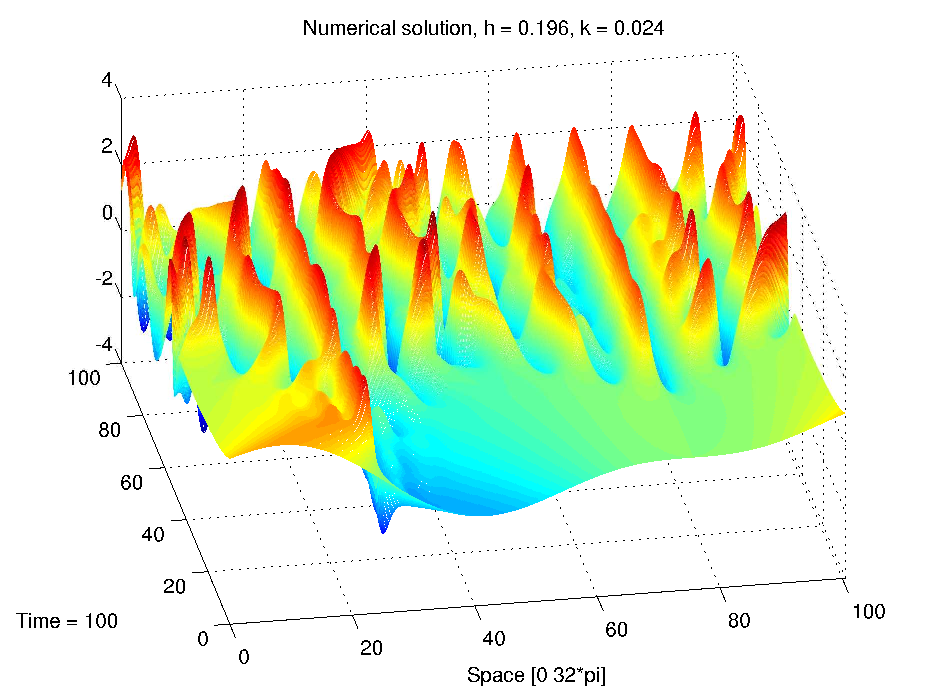
\includegraphics[scale=0.7]
{../PDFs/IMEX/KS_plot_surface.pdf}
\caption{Surface plot of the solution u(x,t)}
\label{fig:surface}
\end{figure}

It is possible to see two parallel lines where the solution is symmetric in an interval around them. This is easier seen from the contour plot, figure \ref{fig:contour}.

\begin{figure}[H]
\centering
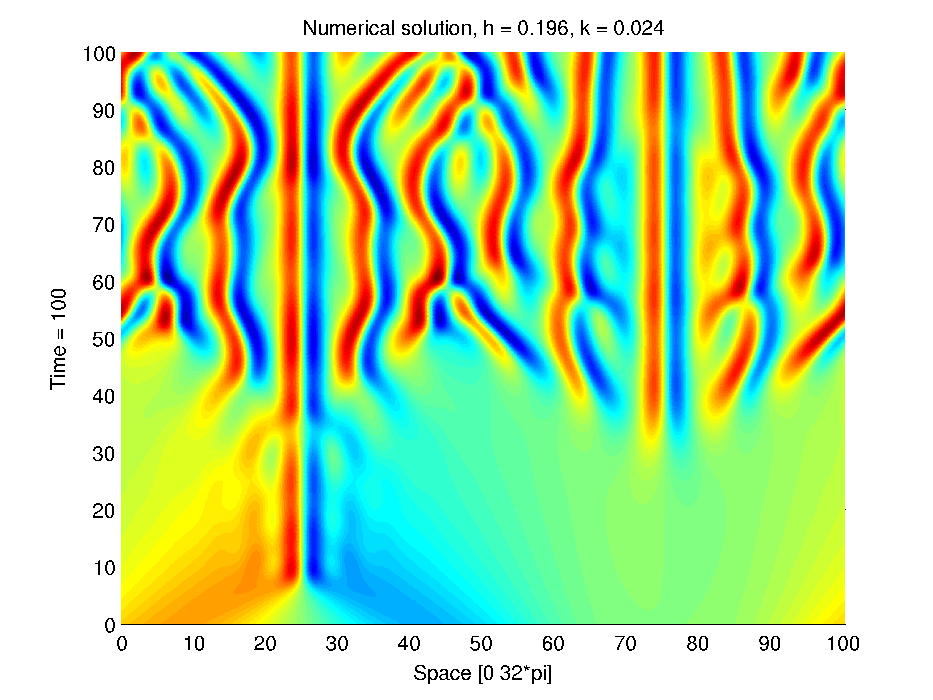
\includegraphics[scale=0.65]
{../PDFs/IMEX/KS_plot_contour.pdf}
\caption{Contour plot of the solution u(x,t)}
\label{fig:contour}
\end{figure}

Although the two lines are parallel at the time interval $t = [0,100]$, this ends after a time $t \thickapprox 250$, and it becomes even more chaotic.

To see exactly how well the numerical solution is compared to the reference solution, we plotted the error between them. Low values for $k$ and $h$ were used for the reference solution, in this case $k = 0.012$ and $h = 0.025$. This produced figure \ref{fig:errPlots}.

\begin{figure}[H]
        \centering
        \begin{subfigure}[b]{0.52\textwidth}
                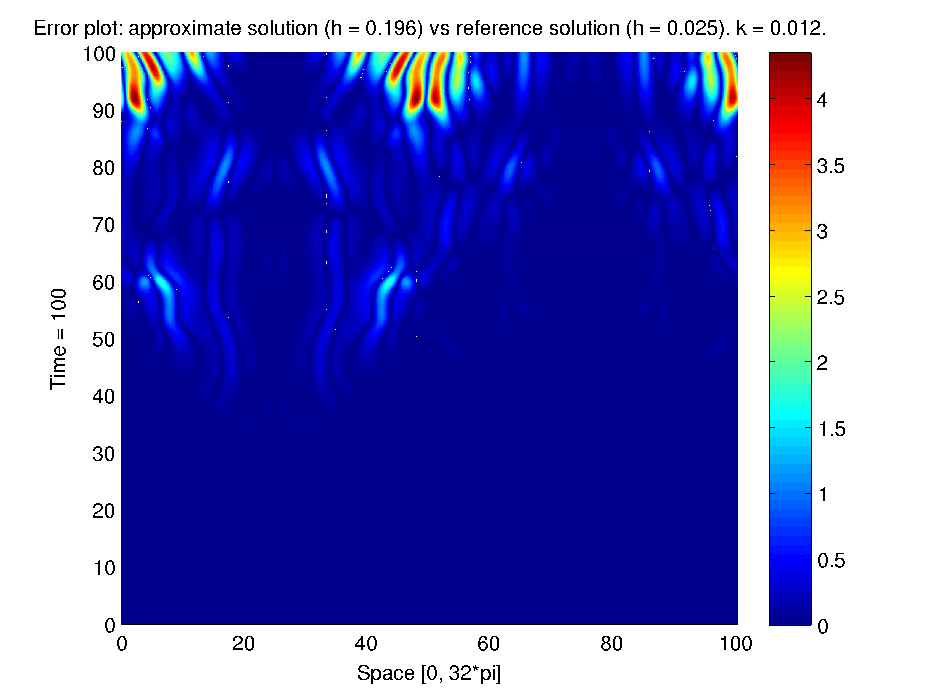
\includegraphics[width=\textwidth]{../PDFs/IMEX/errPlots_worst_scaled.pdf}
                \caption{Error plot of reference vs. numerical, $h = 0.196$ for numerical solution.}
                \label{fig:highError}
        \end{subfigure}%
        ~ %add desired spacing between images, e. g. ~, \quad, \qquad etc.
          %(or a blank line to force the subfigure onto a new line)
        \begin{subfigure}[b]{0.52\textwidth}
                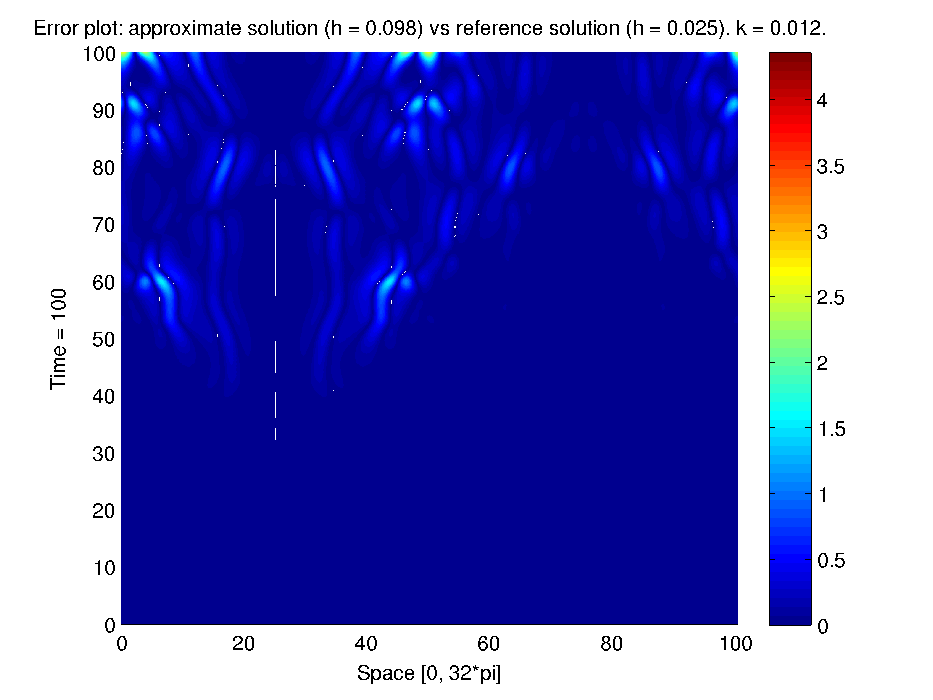
\includegraphics[width=\textwidth]{../PDFs/IMEX/errPlots_best_scaled.pdf}
                \caption{Error plot of reference vs. numerical, $h = 0.098$ for numerical solution.}
                \label{fig:lowError}
        \end{subfigure}
        \caption{Comparison of the error between the reference solution and the numerical approximation for different $h$-values. Reference solution: $h = 0.025$, $k = 0.012$.}\label{fig:errPlots}
\end{figure}

As we can see, the error decreases when the $h$-value is decreased, which is expected. A plot of the reference solution vs. our numerical solution at a given time $t$, figure \ref{fig:errTime}, explains in a good way why some points have larger error than others. At the points where the reference solution are at its maximum and the numerical solution are at its minimum, or vice versa, the error will naturally be large. This means a worst case error will be the sum of the amplitudes of the solutions, and this tends to happen in the chaotic areas. Worth noting is the good approximation at the two parallel lines, $x \thickapprox 25$ and $x \thickapprox 75$, which can also be seen in figure \ref{fig:errPlots}. 

\begin{figure}[H]
\centering
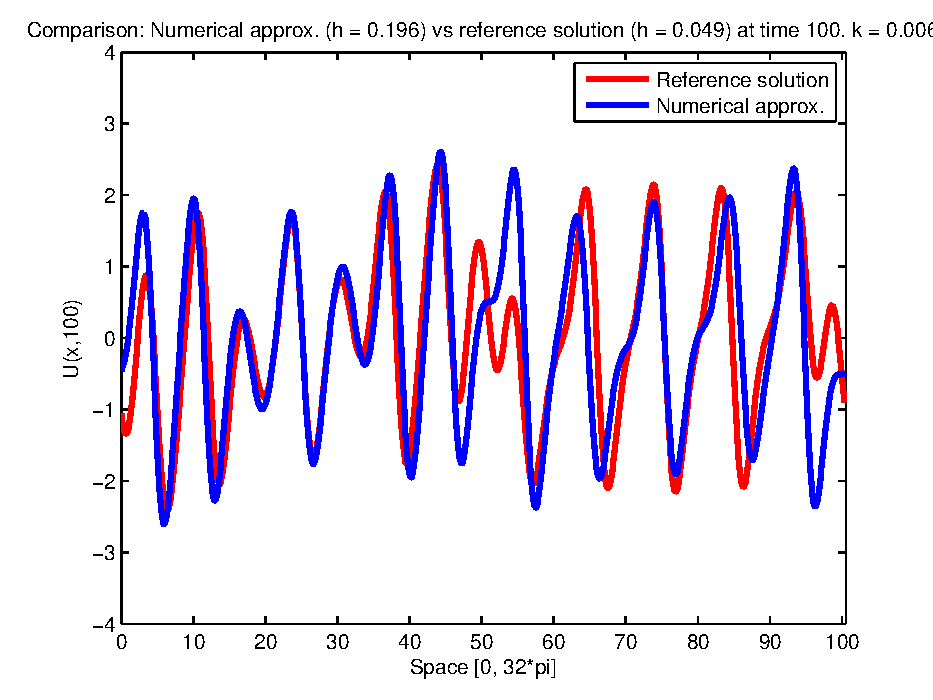
\includegraphics[scale=0.55]
{../PDFs/IMEX/comp_num_ref_t100.pdf}
\caption{Plot of $u(x,100)$ for the reference solution and the numerical solution}
\label{fig:errTime}
\end{figure}

\subsection{Convergence}
\subsubsection{Explicit}
From the analysis, the explicit scheme is consistent, and the local truncation error is $O(k + h^2)$. It is therefore expected that the order of convergence is 1 in time, and 2 in space. Figure \ref{fig:convFE_time} confirms that the order of convergence is 2 in space. However, showing that the order of convergence is 1 in time is not so easy. The constraint $k/h^4 < \frac{1}{8}$ from the analysis of the linearized explicit scheme makes it close to impossible. 

When checking convergence in time, it is important to let the step length in space, $h$, be very small, so the error in space is minimized. This leads to the use of incredibly small step lengths in time. In our attempt at proving the convergence, the infinity norm was constant, with no improvement in the error. The reason for this was that even though the step size was gradually decreased in time, the error in space dominated. Hence a decrease in the error was impossible to see. Because of the constraint, decreasing the step size in space was impossible.

 %EXPLICIT CONVERGENCE PLOT
 
\begin{figure}[H]
\centering
\includegraphics[scale=0.55]
{../PDFs/FE_Exp/expl_time_conv.pdf}
\caption{Convergence in space of order 2}
\label{fig:convFE_time}
\end{figure} 

\subsubsection{Implicit}
The analysis for the implicit scheme showed convergence 2 in space, and 1 in time, as well. It was much easier showing the convergence here, because it's numerically stable. In figure \ref{fig:convergence} one can see that it coincides with the analysis.

 %IMPLICIT CONVERGENCE PLOT
\begin{figure}[H]
        \centering
        \begin{subfigure}[b]{0.52\textwidth}
                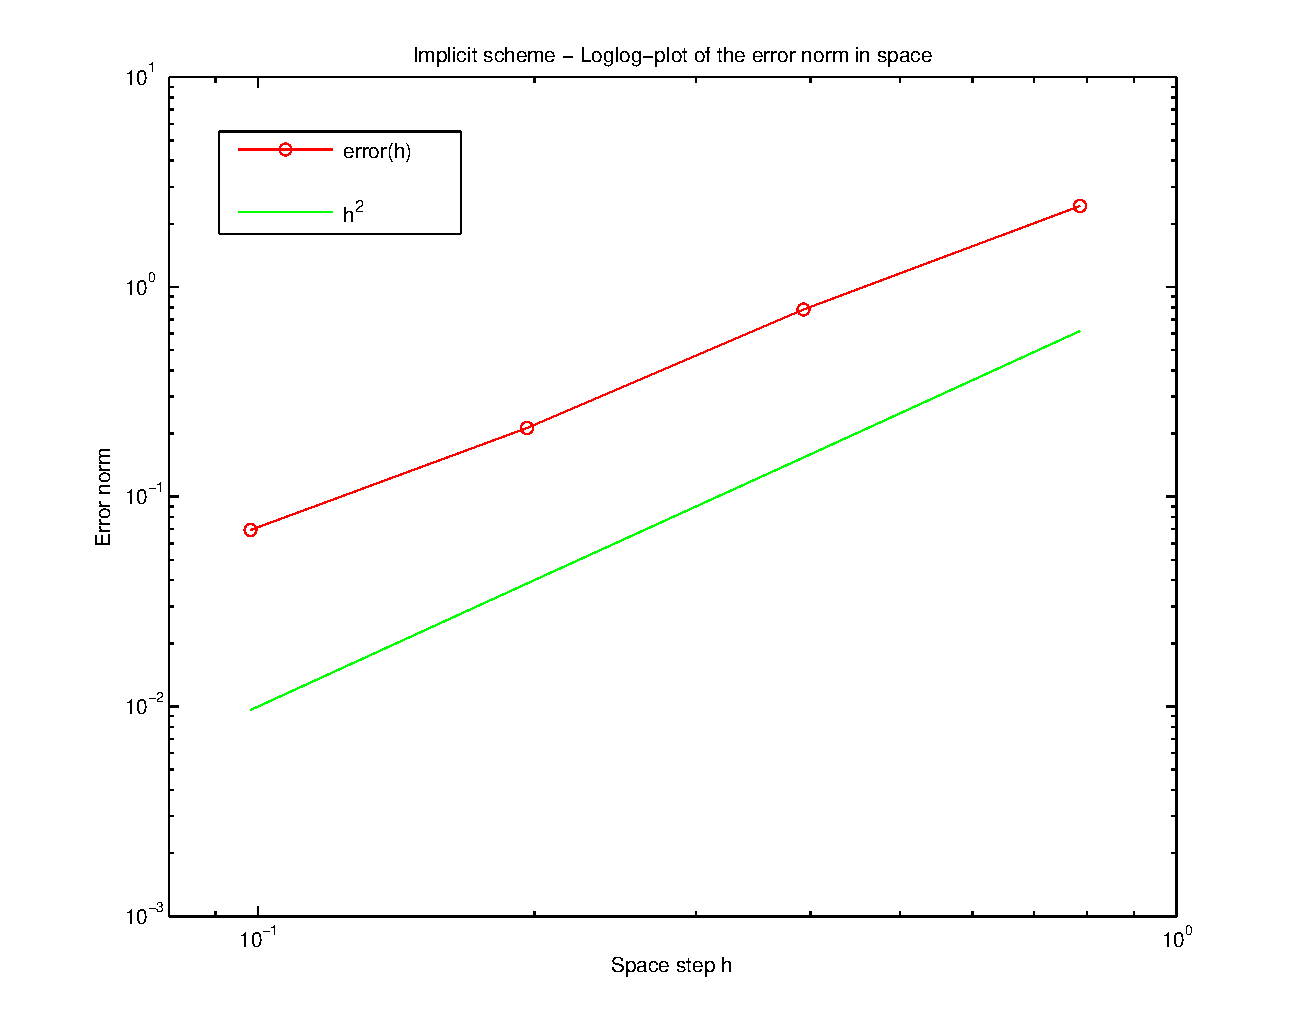
\includegraphics[width=\textwidth]{../PDFs/IMEX/IMEX_space_conv.pdf}
                \caption{Convergence in space of order 2}
                \label{fig:convSpace}
        \end{subfigure}%
        ~ %add desired spacing between images, e. g. ~, \quad, \qquad etc.
          %(or a blank line to force the subfigure onto a new line)
        \begin{subfigure}[b]{0.52\textwidth}
                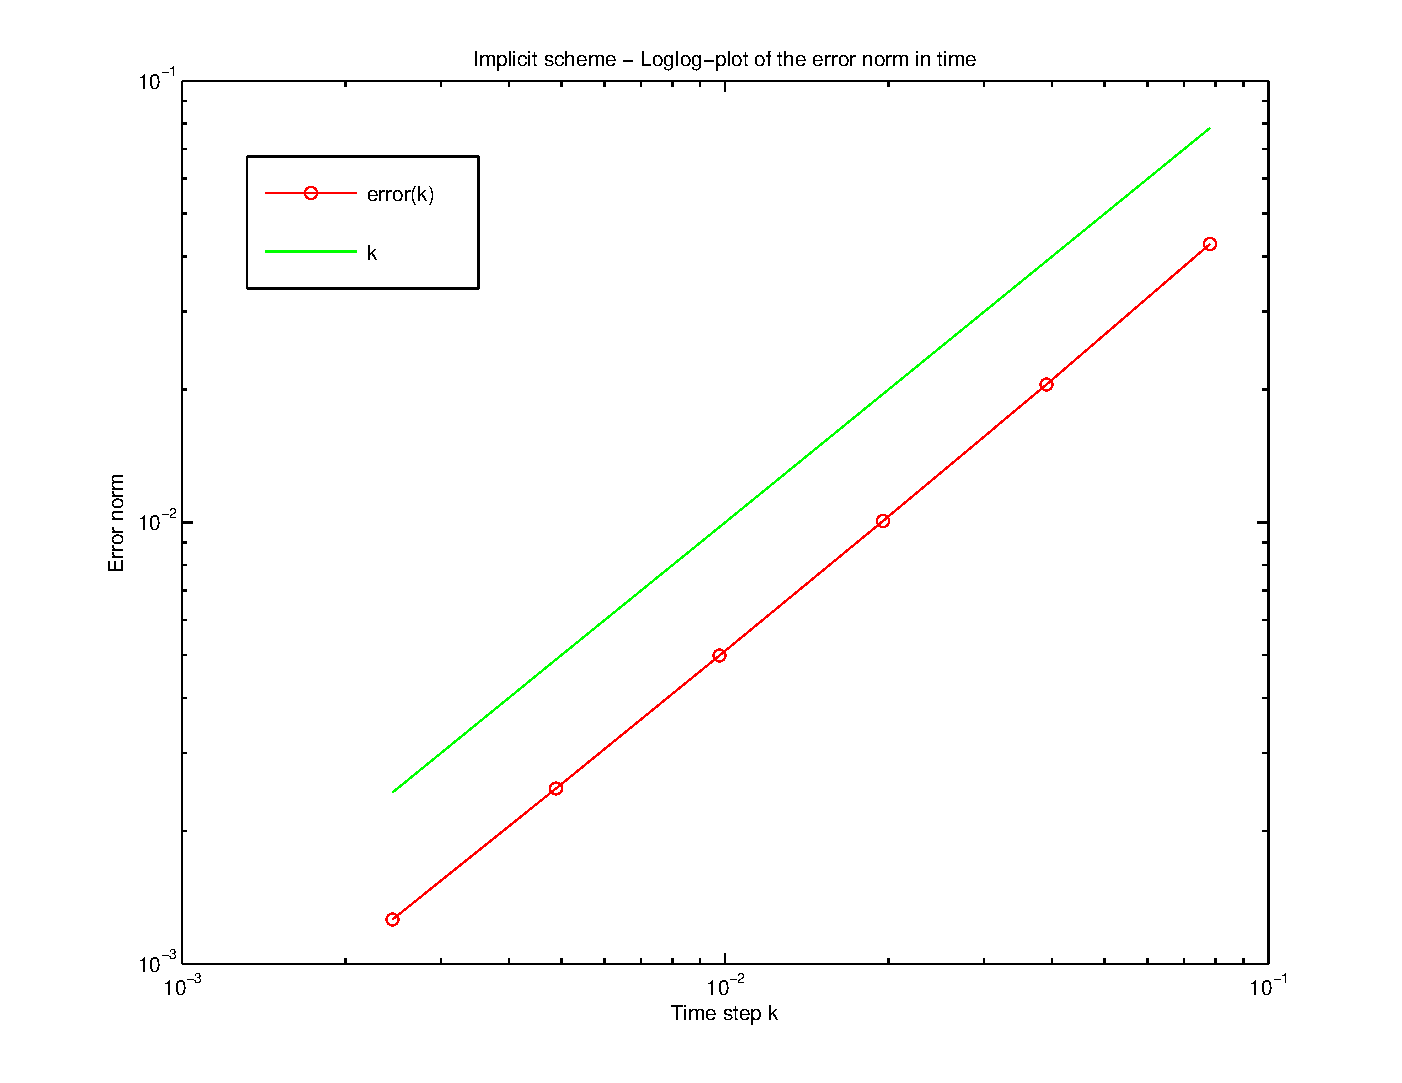
\includegraphics[width=\textwidth]{../PDFs/IMEX/IMEX_time_conv.pdf}
                \caption{Convergence in time of order 1}
                \label{fig:convTime}
        \end{subfigure}
        \caption{Loglog-plots proving convergence in space of order 2, and convergence in time of order 1 for the IMEX-scheme. The green line is the slope.}\label{fig:convergence}
\end{figure}

\subsection{Running time}
In the implementations of both the implicit and the explicit scheme all matrices were implemented using the spdiags-function in MATLAB, which creates sparse band matrices. This is memory efficient, as MATLAB only stores the non-zero elements and their indices. In addition to this, the operations are more computationally efficient than operations on full matrices. \cite{sparse}

To solve the system \eqref{implDiff}, the backslash operator in MATLAB was used. This is possibly the best way to solve a linear system in MATLAB.  In a linear equation $Ax = b$, the backslash operator runs a number of tests to check the structure of the matrix $A$. I.e. if the matrix is sparse and banded, a banded solver is run.

The matrix $\left( I + \frac{k}{2h^2}A + \frac{k}{2h^4}A^2\right)$ from \eqref{implDiff} is a symmetric circular matrix, which is a special kind of Toeplitz matrix where each element is rotated one element to the right relative to the preceding row vector. The advantage of this is that it can be diagonalized by a discrete Fourier transform, such that the implicit scheme can be solved using fast Fourier transform in MATLAB.

The implicit and explicit scheme both have negative and positive properties. While the explicit scheme is about 10 times faster than the implicit scheme, as shown in Figure \ref{fig:runTime}, it has a restriction on the time step that makes it very hard to work with. In addition, it seems that the error is larger in the explicit scheme than the implicit scheme, independent of the number of time steps.

\begin{figure}[H]
        \centering
        \begin{subfigure}[b]{0.52\textwidth}
                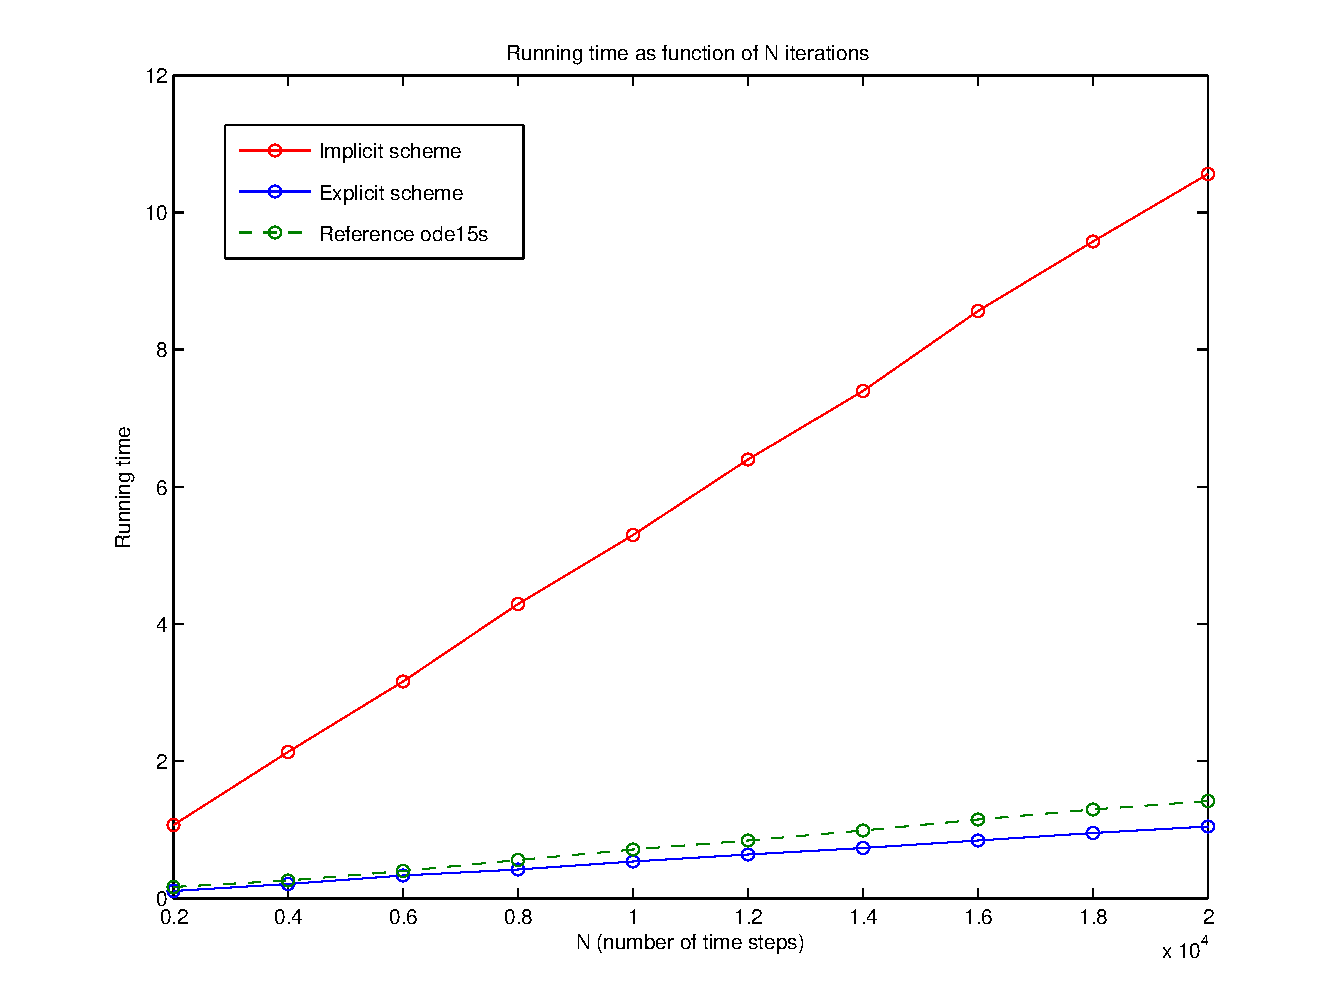
\includegraphics[width=\textwidth]{../PDFs/Comparisons/running_time3.pdf}
                \caption{Running time of the two schemes as a function of time steps $N$}
                \label{fig:runTime}
        \end{subfigure}%
        ~
        \begin{subfigure}[b]{0.52\textwidth}
                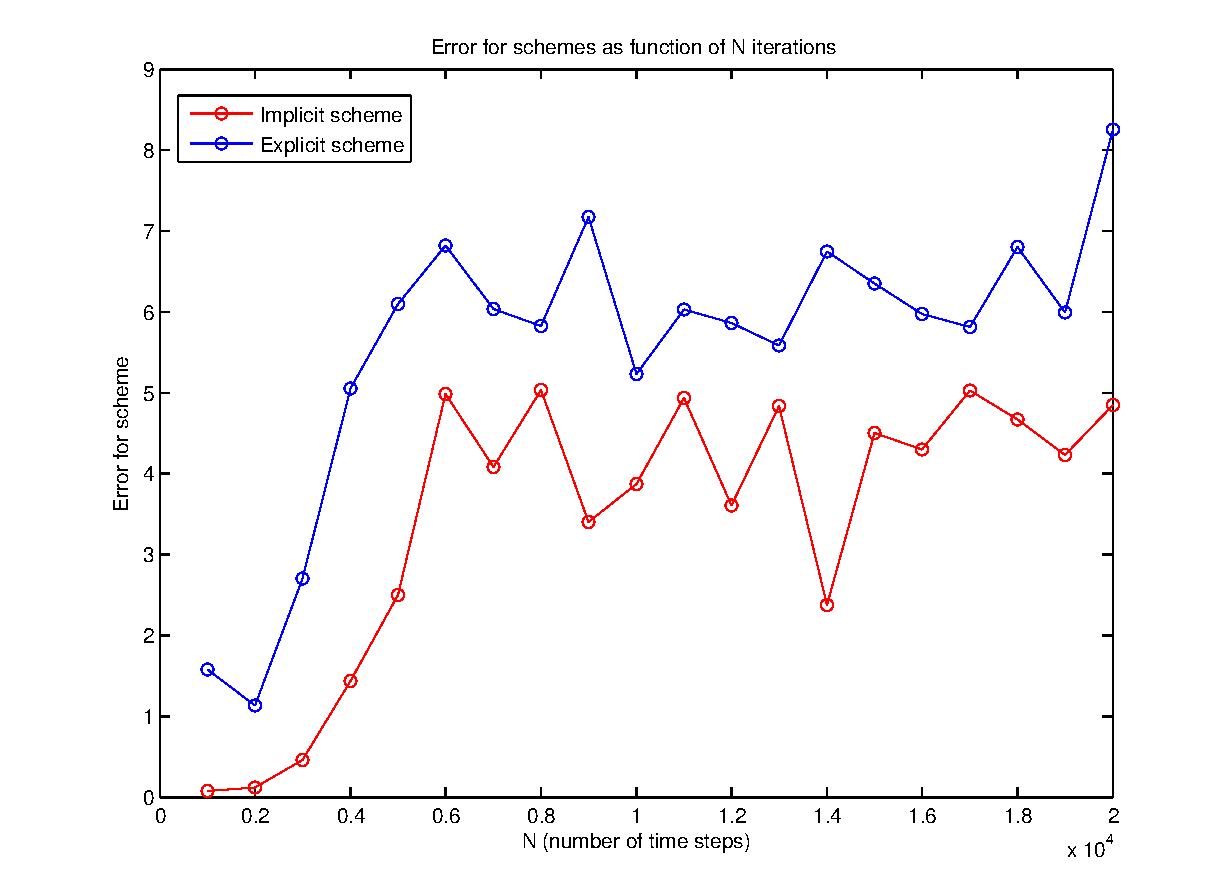
\includegraphics[width=\textwidth]{../PDFs/Comparisons/error_compare.pdf}
                \caption{Global error of the two schemes as a function of time steps $N$}
                \label{fig:solImp}
        \end{subfigure}
        \caption{Comparisons of the explicit method and the IMEX-method.}
        \label{fig:runTimeN}
\end{figure}

In an attempt to make the program more efficient for solving our linear system, LU-decomposition was implemented using MATLAB's lu()-function. However, this did not result in better running times for our algorithm. A hypothesis for this is that MATLAB's backslash operator is very efficient for solving systems with sparse matrices, so that our system of sparse matrices is solved in minimal running time. Though a LU-decomposition is an efficient way of solving linear systems, it does not weigh out adding a backslash operation to the code.

Newton's method was implemented to get consistency of second order in time. Though this was more efficient than solving the implicit scheme, the solution was not satisfying, as can be seen from Figure \ref{fig:solNewton} and Figure \ref{fig:solImp}. When comparing these with the reference solution, we must conclude that the solution produced by Newton's method does not give the wanted accuracy, and the improvement in running time does not weigh out for a poor solution.

\begin{figure}[H]
        \centering
        \begin{subfigure}[b]{0.52\textwidth}
                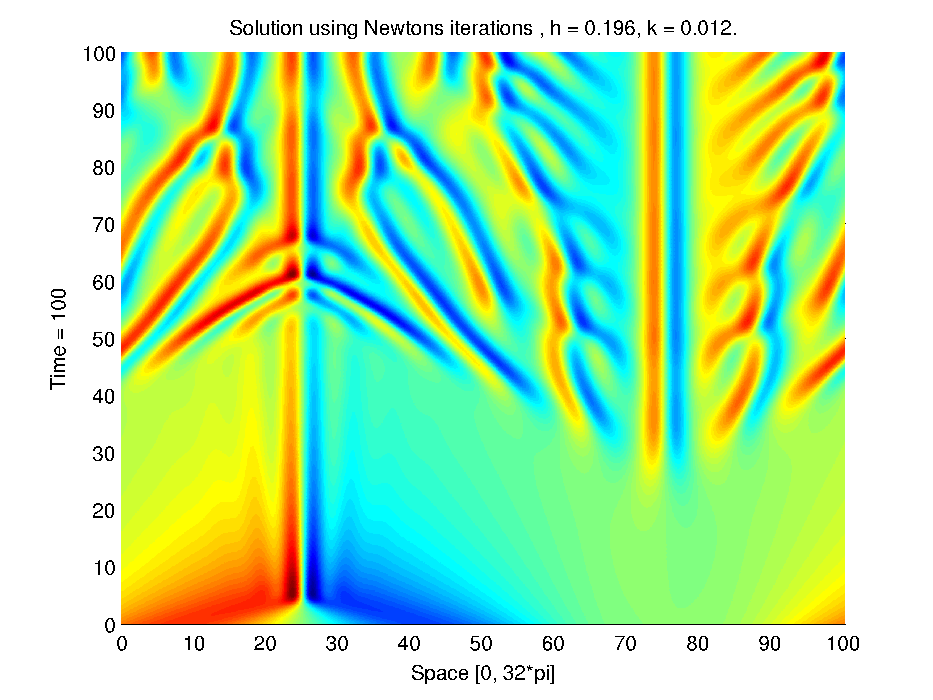
\includegraphics[width=\textwidth]{../PDFs/Comparisons/SolNewton.pdf}
                \caption{Solution using Newton's method}
                \label{fig:solNewton}
        \end{subfigure}%
        ~
        \begin{subfigure}[b]{0.52\textwidth}
                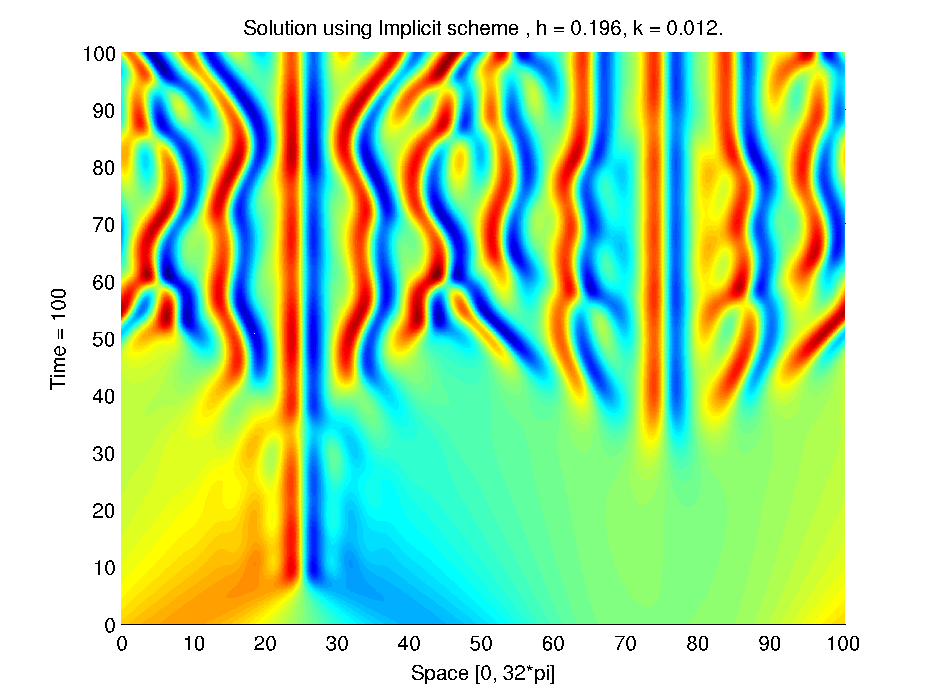
\includegraphics[width=\textwidth]{../PDFs/Comparisons/SolImp.pdf}
                \caption{Solution using IMEX method}
                \label{fig:solImp}
        \end{subfigure}
        \caption{Comparison of the solution by using the IMEX-method and Newton's method.}
        \label{fig:compNewtImpl}
\end{figure}

%\begin{figure}[H]
%\centering
%\includegraphics[scale=0.4]
%{../PDFs/Comparisons/running_time3.pdf}
%\caption{Running time of the two schemes as a function of time steps $N$}
%\label{fig:runTime}
%\end{figure}
%
%\begin{figure}[H]
%\centering
%\includegraphics[scale=0.4]
%{../PDFs/Comparisons/error_compare.pdf}
%\caption{Global error of the two schemes as a function of time steps $N$}
%\label{fig:runTime}
%\end{figure}